\chapter{Présentation du Sujet de Stage}

\section{Présentation du sujet de stage}
	\textbf{Sujet :}
	
	Développement d'un systeme workflow en cloud computing. Accompagnement d'un audit de sécurité
	
	\textbf{Description :}
	
Deux parties composent le stage :

Au sein du centre de service partagés d'Annemasse composé de 5 sites (Abbeville, Mondeville, Créteil, Ben Arous, Annemasse), le développement d'un ensemble d'applications sous deux environnements en cloud computing (Google Apps et google script, et Cordys). \\
Pour cette partie, les objectifs sont : 
\begin{enumerate}
	\item Déployer un plan d'action pour qualifier, planifier, développer et mettre en production un ensemble d'applications intégrant du workflow sur un environnement Cordys (processus de gestion de workflow)
	\item Utiliser et développer les évolutions des modèles de Google Site et Google Scripts sur un parc applicatifs existant
	\item Planifier et ordonnancer les lancements de mise en productions avec les Business Owners
\end{enumerate}
\vspace{6mm}

Au sein du site d'Annemasse, aider à la préparation d'un audit de sécurité informatique du site organisé par le Groupe.
Pour cette partie, les objectifs sont :
\begin{enumerate}
	\item Le développement de scripts de contrôle au niveau du réseau
	\item La préparation d'une documentation
	\item L'accompagnement dans le projet dans les démarches sécuritaires (opérations techniques, et communications aux users)
\end{enumerate}
\vspace{6mm}

L'ensemble des actions menées durant le stage devront être réalisées dans une démarche industrielle devant respecter les contraintes Coûts /Qualité / Délais. 

Des qualités de communication sont requises (français maîtrisé/ anglais parlé) car les contacts avec la Direction sont fréquents. Des déplacements pourront être envisagés dans le cadre du stage. 


\section{Fiche de Poste}
 \begin{figure}[H]
    \centering
    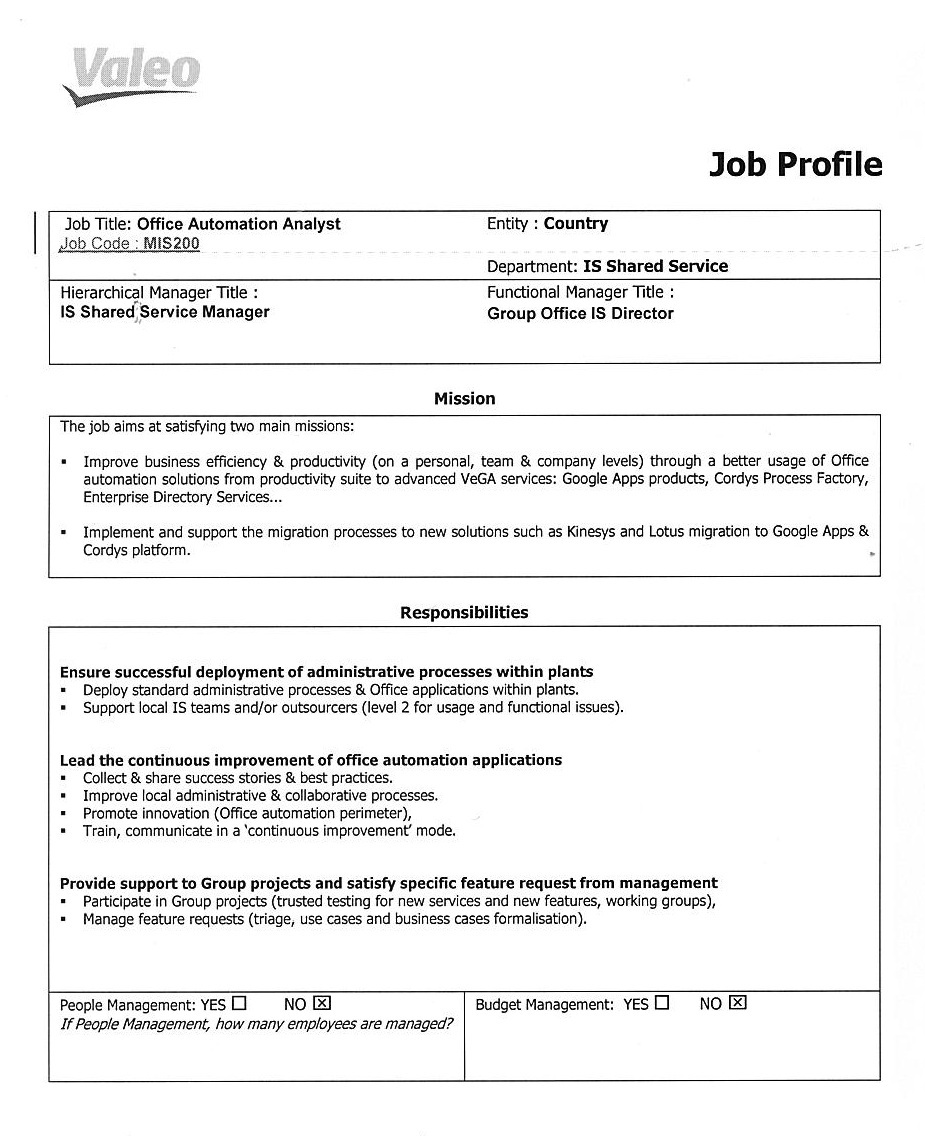
\includegraphics[height=22cm]{job_profil.jpg}
	\caption{Fiche de poste}\label{image.jobprofil} 
\end{figure} 

\clearpage
